\section{Resultados}
\label{sec:resultados}

Todas las figuras de esta sección usan retratos oficiales de la NASA, de dominio público. Durante el desarrollo, los cortes y el tinte de barba se revisaron también sobre 19 caras variadas de CelebAMask-HQ, que no se reproducen aquí por licencia.

\subsection{Cortes de pelo}

La figura~\ref{fig:cortes} muestra los ocho cortes sobre tres personas con pelo distinto: liso y oscuro, afro, y castaño claro. En todos los casos el fondo detrás del pelo quitado queda limpio, sin pelo fantasma, y la cara no cambia. Cada degradado muestra la piel a una altura distinta:
\begin{itemize}
  \item el \emph{taper} conserva pelo corto hasta abajo;
  \item el \emph{undercut} afeita los costados de forma plana bajo un borde duro;
  \item la raya marcada agrega la línea afeitada entre la parte de arriba y el costado;
  \item el \emph{crew cut} y el rapado reemplazan todo el volumen por pelo corto del color de la persona, con la línea del pelo tomada de su frente.
\end{itemize}

\begin{figure}[ht]
  \centering
  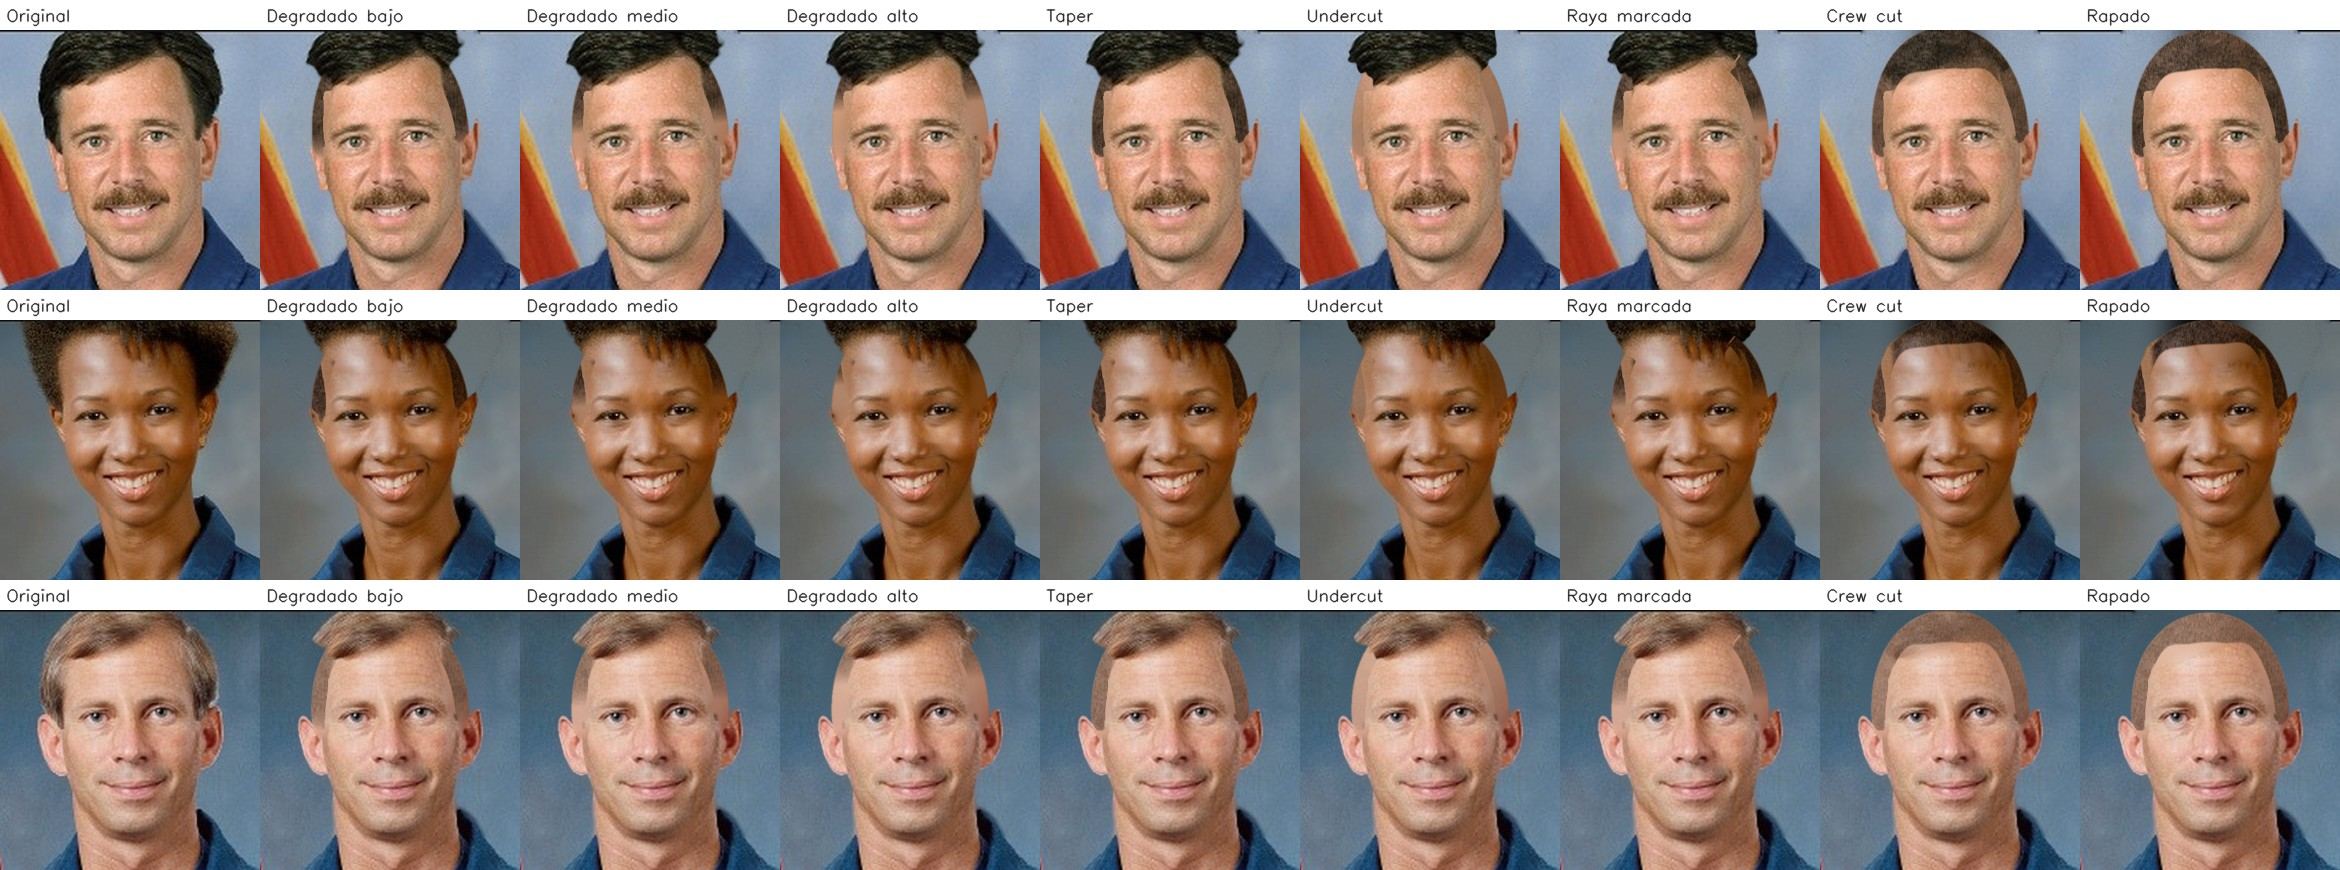
\includegraphics[width=\linewidth]{cortes.jpg}
  \caption{Los ocho cortes sobre tres retratos de dominio público.}
  \label{fig:cortes}
\end{figure}

\subsection{Tinte y segmentación del pelo}

La figura~\ref{fig:tinte} compara las máscaras del YOLO propio y de MediaPipe, y el tinte con cada una:
\begin{itemize}
  \item las dos máscaras coinciden en la mayor parte del pelo;
  \item el YOLO propio tiende a incluir más borde y más mechones finos.
\end{itemize}
Medida como IoU entre las máscaras sin refinar, la coincidencia fue de 0{,}82 a 0{,}94 en siete retratos de prueba. Dentro de la aplicación, que compara la máscara refinada de YOLO con la de MediaPipe, el valor reportado varió entre 0{,}58 (pelo muy corto y rizado) y 0{,}96. El tinte conserva la textura del pelo y logra tanto aclarar como oscurecer.

\begin{figure}[ht]
  \centering
  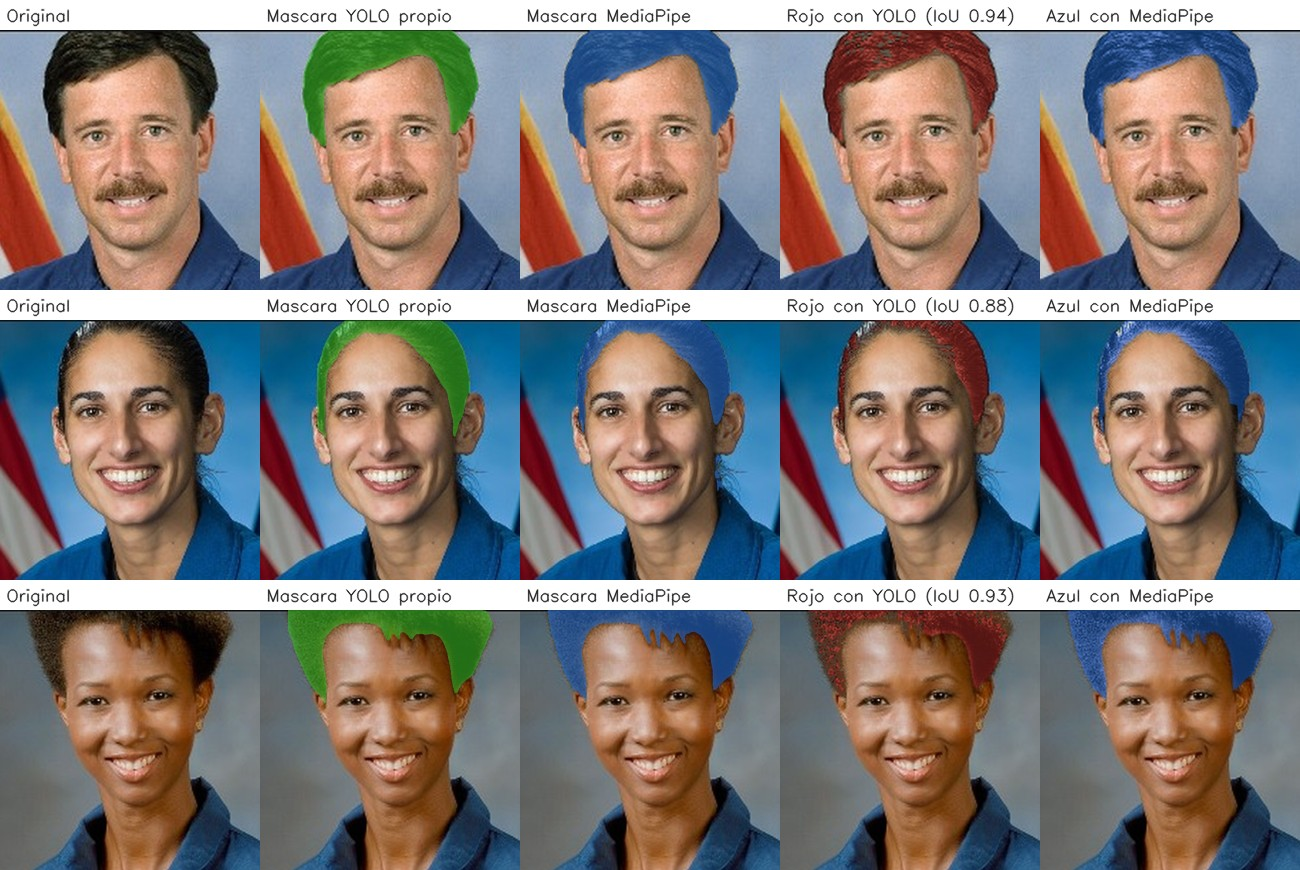
\includegraphics[width=0.95\linewidth]{tinte_modelos.jpg}
  \caption{Máscara del YOLO propio (verde) y de MediaPipe (azul), y el tinte con cada una. El título de la cuarta columna indica la IoU entre ambas máscaras.}
  \label{fig:tinte}
\end{figure}

\subsection{Tinte de la barba}

La figura~\ref{fig:barbatinte} muestra el tinte de barba en dos casos: una barba puesta por la propia aplicación, que se tiñe entera usando la máscara de su estilo, y un bigote real, detectado por textura.

\begin{figure}[ht]
  \centering
  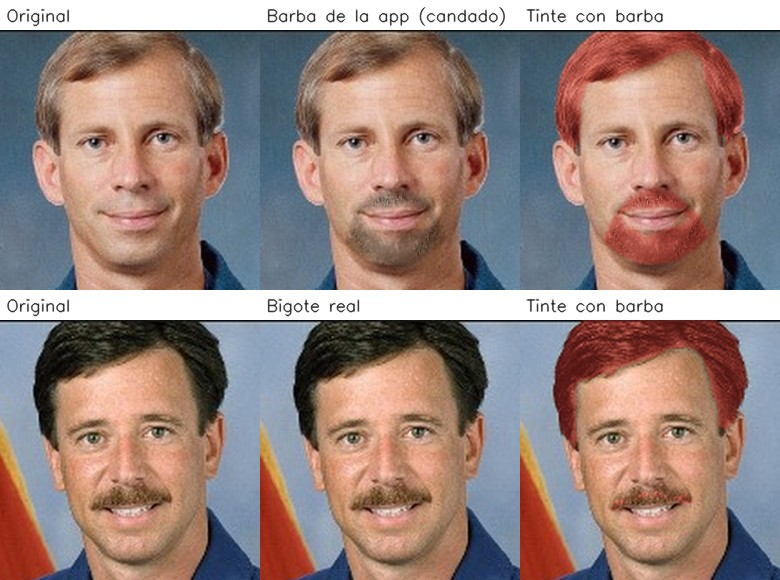
\includegraphics[width=0.62\linewidth]{barba_tinte.jpg}
  \caption{Tinte de barba. Arriba, un candado puesto por la aplicación; abajo, un bigote real.}
  \label{fig:barbatinte}
\end{figure}

\subsection{Gaussianas 2D}

La tabla~\ref{tab:psnr} resume la calidad de la reconstrucción en seis retratos. La relación señal/ruido de pico (PSNR) crece casi linealmente con $\log N$: unos 8~dB por cada multiplicación por diez del número de gaussianas (figura~\ref{fig:psnr}).

\begin{table}[ht]
\centering
\small
\begin{tabular}{@{}rccc@{}}
\toprule
Gaussianas & PSNR medio (dB) & Rango (dB) & Tiempo medio (s) \\
\midrule
20 & 18{,}4 & 16{,}7 -- 20{,}2 & 0{,}9 \\
60 & 22{,}2 & 20{,}3 -- 24{,}9 & 2{,}4 \\
200 & 26{,}0 & 24{,}1 -- 28{,}4 & 4{,}1 \\
600 & 29{,}8 & 27{,}5 -- 31{,}8 & 3{,}8 \\
2000 & 34{,}5 & 32{,}9 -- 35{,}9 & 3{,}6 \\
\bottomrule
\end{tabular}
\caption{Reconstrucción de retratos con gaussianas 2D.}
\label{tab:psnr}
\end{table}

\begin{figure}[ht]
  \centering
  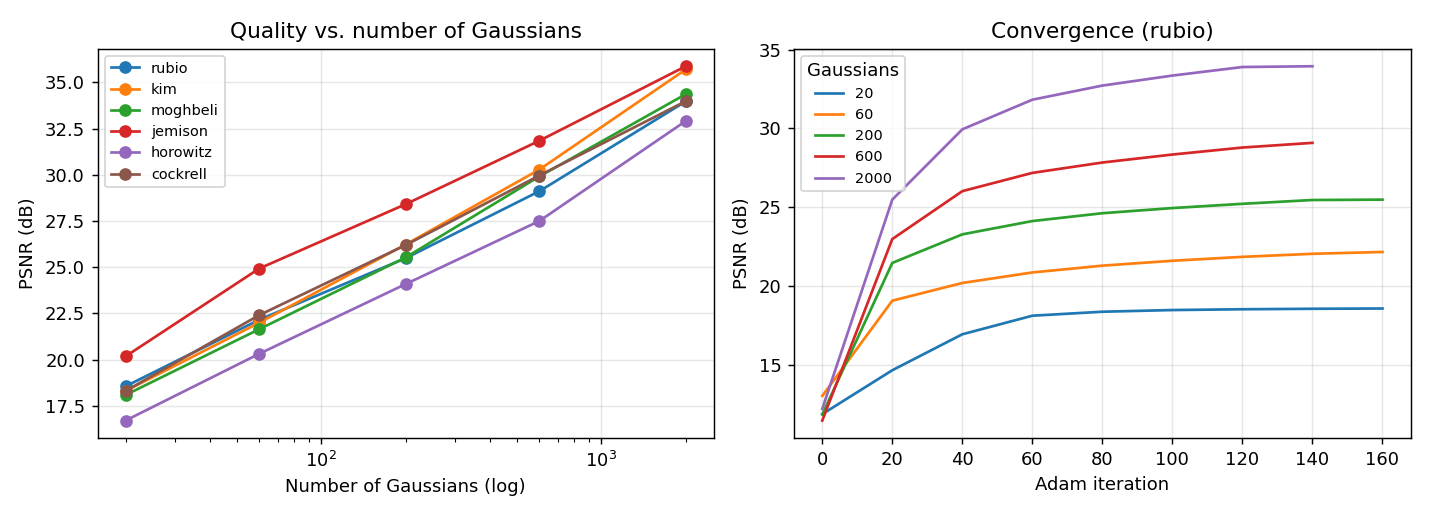
\includegraphics[width=0.85\linewidth]{psnr.png}
  \caption{PSNR en función del número de gaussianas y convergencia por iteración.}
  \label{fig:psnr}
\end{figure}

\subsection{Contrarreloj}

Para validar el juego se programó un ``bot barbero'' que recorre en zigzag la zona que hay que afeitar y levanta la máquina en los saltos largos (tabla~\ref{tab:juego}). Un bot que corta sin levantar la máquina, cruzando el objetivo, obtiene 0~puntos. Esto confirma que el puntaje premia afeitar con cuidado.

\begin{table}[ht]
\centering
\small
\begin{tabular}{@{}lccc@{}}
\toprule
Retrato y objetivo & Puntaje & Limpieza & Conservación \\
\midrule
rubio, candado & 827 & 0{,}83 & 0{,}99 \\
rubio, bigote & 814 & 1{,}00 & 0{,}81 \\
rubio, collar & 690 & 0{,}69 & 1{,}00 \\
kim, candado & 817 & 0{,}83 & 0{,}99 \\
horowitz, collar & 656 & 0{,}66 & 1{,}00 \\
cockrell, bigote & 646 & 0{,}98 & 0{,}66 \\
\bottomrule
\end{tabular}
\caption{Resultados del bot barbero.}
\label{tab:juego}
\end{table}

\subsection{Interfaz}

La interfaz (figuras~\ref{fig:inicio}, \ref{fig:ui} y~\ref{fig:ficha}) organiza las herramientas en cuatro grupos: \emph{Estilos}, \emph{3D}, \emph{Juegos} y \emph{Mis looks}. La foto es compartida entre todas las herramientas y cada resultado se ve en un comparador antes/después. La tarjeta ``Tu cara'' muestra la forma detectada y marca los estilos sugeridos. La interfaz se adapta al celular.

\begin{figure}[ht]
  \centering
  \begin{subfigure}{0.49\linewidth}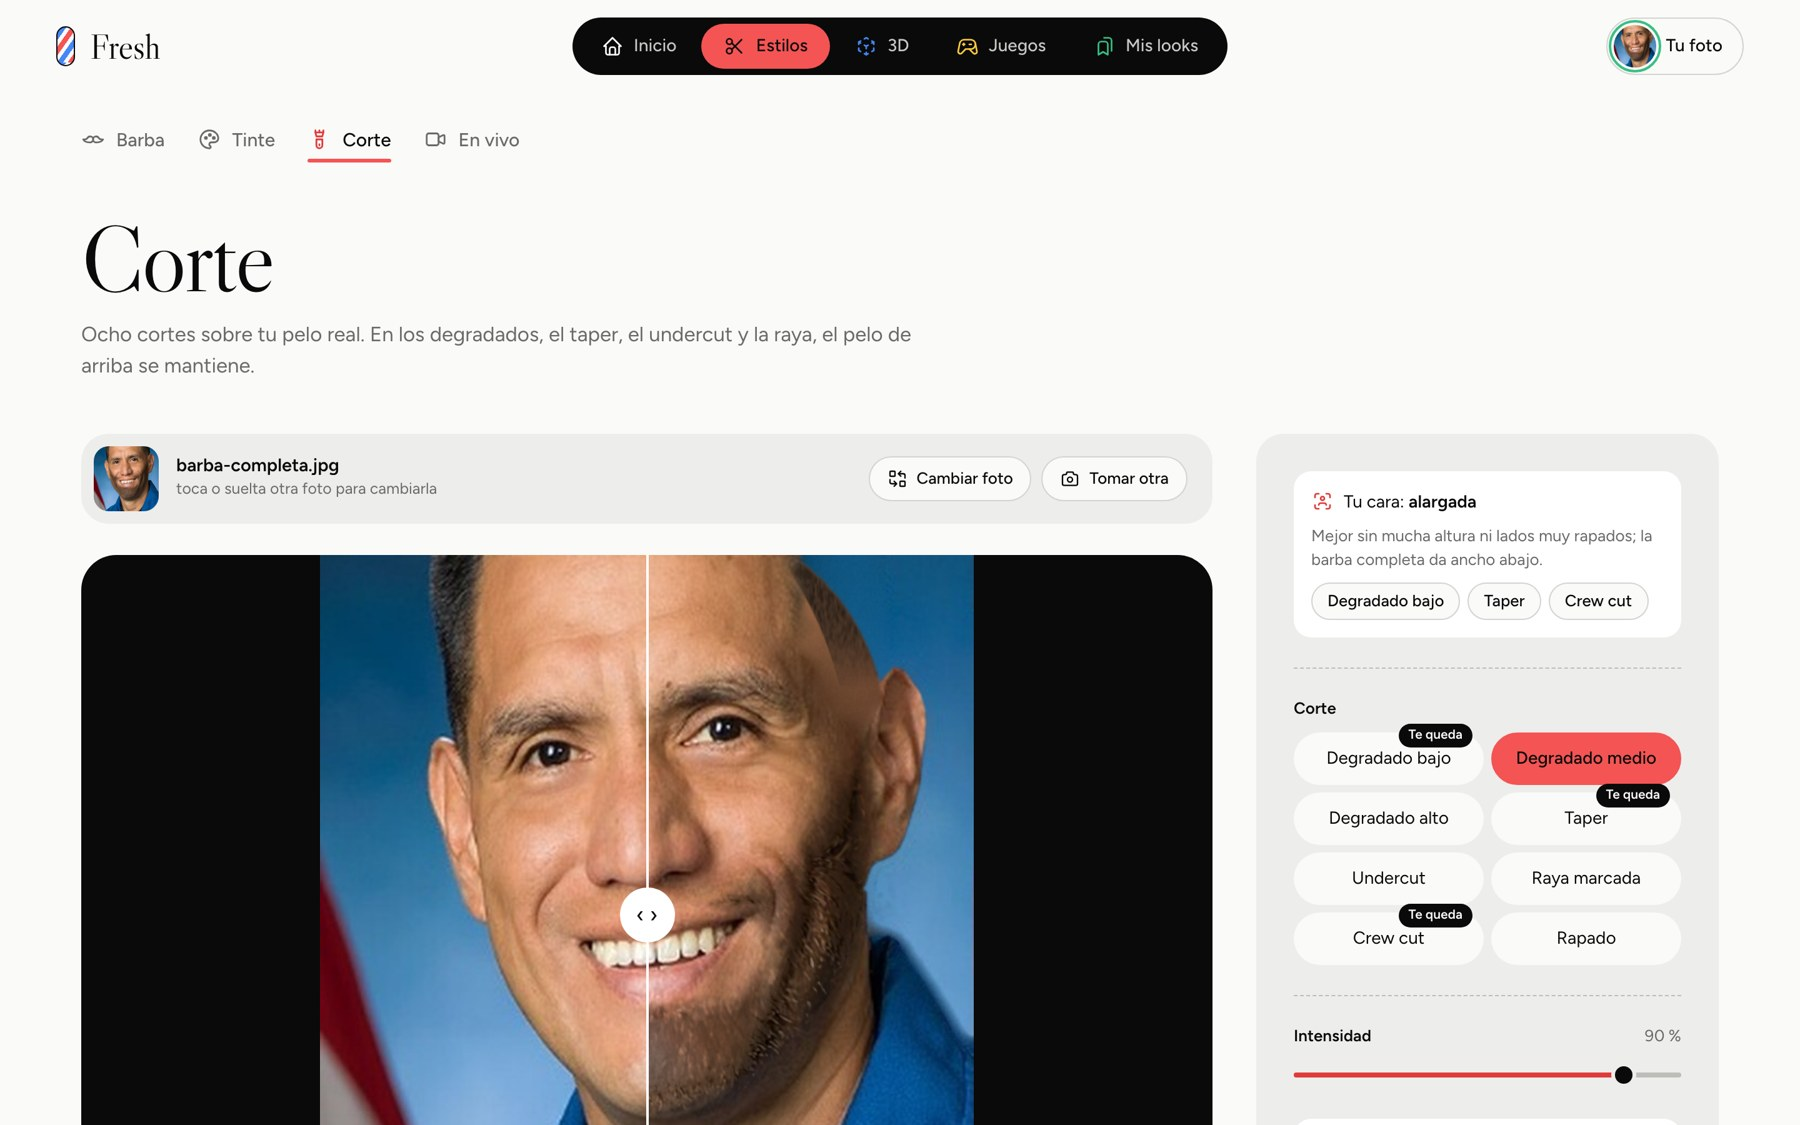
\includegraphics[width=\linewidth]{ui_corte.jpg}\caption{Corte, con sugerencias por forma de cara}\end{subfigure}\hfill
  \begin{subfigure}{0.49\linewidth}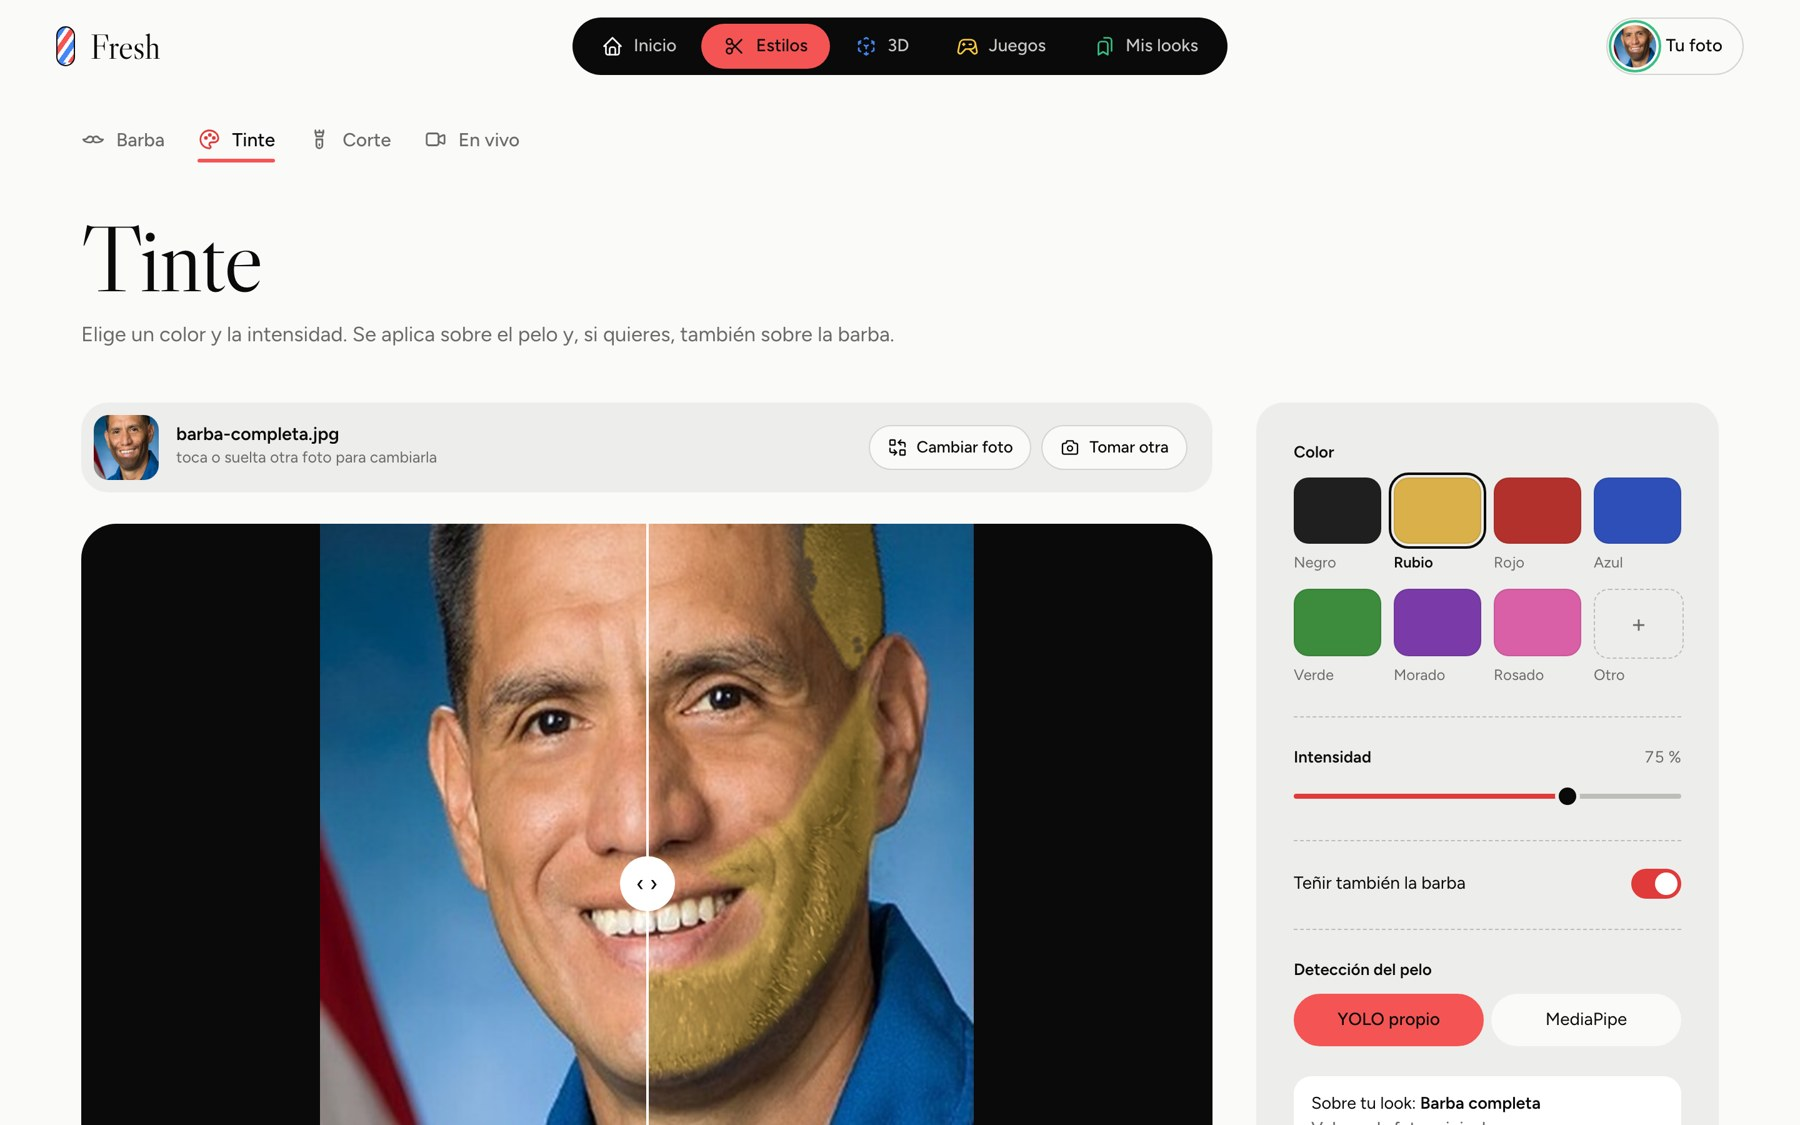
\includegraphics[width=\linewidth]{ui_tinte.jpg}\caption{Tinte con barba y selector de modelo}\end{subfigure}
  \caption{Paneles de Corte y Tinte sobre un look combinado.}
  \label{fig:ui}
\end{figure}

\begin{figure}[ht]
  \centering
  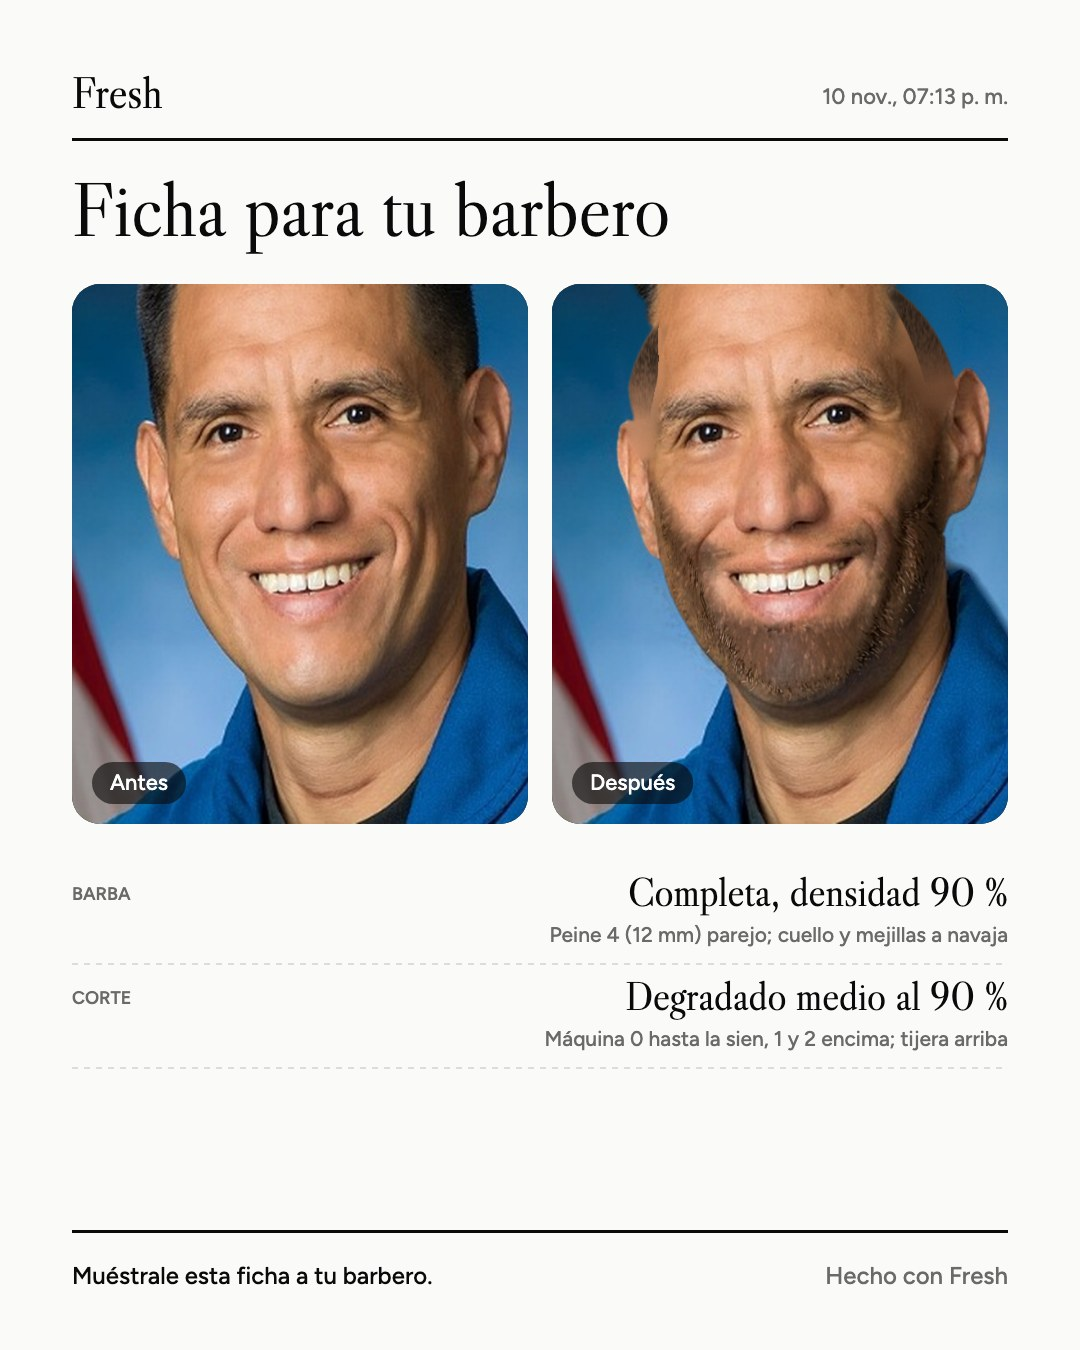
\includegraphics[width=0.45\linewidth]{ui_ficha.jpg}
  \caption{Ficha para el barbero de un look combinado, con indicaciones de máquina por servicio.}
  \label{fig:ficha}
\end{figure}

\subsection{Rendimiento}

La tabla~\ref{tab:tiempos} reúne los tiempos medidos. Las fotos más grandes que 2048~px se reducen al recibirlas: una foto de 4000~px tardaba 18~s en el contenedor y ahora tarda menos de 1~s.

\begin{table}[ht]
\centering
\small
\begin{tabularx}{\linewidth}{@{}X r@{}}
\toprule
Operación & Tiempo \\
\midrule
Corte, fotos de 1024 a 1638~px (contenedor Docker, CPU) & 0{,}6 -- 1{,}9~s \\
Corte, foto de 4000~px (contenedor Docker) & 0{,}8 -- 1{,}1~s \\
Corte, foto de 600~px (Apple M5, local) & 0{,}1 -- 0{,}3~s \\
Tinte con YOLO y barba (contenedor Docker, modelo ya cargado) & 2{,}5~s \\
Construcción del espejo 3D (unas 105\,000 gaussianas) & 2{,}6~s \\
Barba en vivo, por cuadro & 61~ms \\
Física de la barba en vivo, por cuadro & 72~ms \\
\bottomrule
\end{tabularx}
\caption{Tiempos medidos.}
\label{tab:tiempos}
\end{table}

\subsection{Pruebas automáticas}
\label{sec:pruebas}

El proyecto tiene 53 pruebas con pytest, que GitHub Actions ejecuta en cada cambio:
\begin{itemize}
  \item 32 de la API y de los módulos de estilo;
  \item 10 de \emph{splatting} y física;
  \item 5 de la transferencia de pelo;
  \item 4 de la triangulación de Delaunay;
  \item 2 del laboratorio.
\end{itemize}

Entre otras cosas, verifican:
\begin{itemize}
  \item \textbf{Delaunay}: ningún punto cae dentro de un círculo circunscrito, hay $2n-2-h$ triángulos, una grilla da exactamente los triángulos esperados sin superposiciones, los puntos colineales no generan triángulos y Fortune contiene todos los triángulos de Bowyer--Watson;
  \item \textbf{cortes}: ningún corte toca la cara; con intensidad 0 la foto no cambia; los píxeles lejos del pelo no cambian; un estilo desconocido da error;
  \item \textbf{entradas inválidas}: sin cara, la API responde 422, y con un estilo o modelo desconocido, 400;
  \item \textbf{forma de la cara}: la clasificación es correcta en proporciones sintéticas y todas las sugerencias corresponden a estilos existentes;
  \item \textbf{tinte de barba}: no tiñe piel limpia;
  \item \textbf{gaussianas 2D}: más gaussianas dan mayor PSNR;
  \item \textbf{física}: se asienta en reposo y se atrasa al mover la raíz;
  \item \textbf{espejo 3D}: las covarianzas son semidefinidas positivas y el \texttt{.ply} reconstruye exactamente la covarianza original;
  \item \textbf{juego}: no corta nada con la máquina apagada y conserva su objetivo entre cuadros;
  \item \textbf{servidor}: corre un solo proceso, para no partir el estado del modo en vivo y del juego.
\end{itemize}
Además, la aplicación arranca y aprueba las pruebas tanto con YOLO instalado como sin él.
